\providecommand{\imgpath}{.}
\documentclass[crop,tikz]{standalone}
\usepackage{graphicx}
\usepackage{color}

\usepackage{listings}
\usepackage{lstautogobble}  % Fix relative indenting
%\usepackage{zi4}            % Nice font

\usepackage{amssymb}
\usepackage{amsmath}

\usepackage{xspace}
\usepackage{hyperref}
\usepackage{multirow}
\usepackage{makecell}
\usepackage[caption=false]{subfig}
\usepackage{booktabs}

\usepackage[mode=buildnew]{standalone}
\usepackage{tikz}
\usetikzlibrary{positioning}
\usetikzlibrary{calc}
\usetikzlibrary{fit}
\usetikzlibrary{shapes.arrows}
\usetikzlibrary{backgrounds}

% JSC packages
\usepackage{soulutf8}
\newcommand{\hlb}[1]{{\sethlcolor{SkyBlue}\hl{#1}}}
%\usepackage{subcaption}

% tabular format
\usepackage{tabularx}
\usepackage{arydshln}
\setlength\dashlinedash{0.2pt}
\setlength\dashlinegap{1.5pt}
\setlength\arrayrulewidth{0.3pt}
\newcommand{\ra}[1]{\renewcommand{\arraystretch}{#1}}

% landscape for yearly tables and sizing
\usepackage{pdflscape}
\usepackage{adjustbox}
\usepackage{float}

\usepackage[T1]{fontenc}

%comment paragraph summary for structure re-engineering
% \usepackage{todonotes}
% \setuptodonotes{color=lightblue!10, linecolor=lightblue, bordercolor=lightblue}

\begin{document}

\begin{tikzpicture}
	\tikzstyle{roundrect} = [rectangle, rounded corners, text centered]
	\tikzstyle{arr} = [single arrow]

	\newcommand\LineWidth{0.3mm}
	\newcommand\ArrowColor{AITturquoise}

	\newcommand\TransformWidth{5cm}
	\newcommand\IngestWidth{3cm}
	\newcommand\SourcesWidth{4cm}
	\newcommand\TransformHeight{5cm}
	\newcommand\LabelShift{-\TransformHeight}
	\newcommand\LedgersLabelShift{-1.1}

	\newcommand\DashboardWidth{2.2cm}
	\newcommand\DashboardHeight{1.8cm}
	\newcommand\DashboardYShift{1.8cm}

	\newcommand\APIWidth{4.75cm}
	\newcommand\APIHeight{.8cm}
	\newcommand\APIYShift{-1cm}

	\newcommand\LedgersWidth{3.6cm}
	\newcommand\BlockSciWidth{2.6cm}
	\newcommand\BlockSciHeight{1cm}
	\newcommand\BlockSciYShift{-1.2cm}

	\newcommand\RawWidth{2cm}
	\newcommand\RawHeight{\TransformHeight / 2}
	\newcommand\RawXShift{-2.15cm}
	\newcommand\CassandraYShift{-.8cm}


	% transformation
	\node [roundrect, fill=AITturquoise, minimum width=\TransformWidth, minimum height=\TransformHeight, label={[shift={(0, \LabelShift)}]Data Transformation and Storage}](transform) at (0, 0) {};

	\node [roundrect, fill=white, left = \RawXShift of transform, minimum width=\RawWidth, minimum height=\RawHeight](raw) {Raw Data};
	\node [roundrect, fill=white, right = \RawXShift of transform, minimum width=\RawWidth, minimum height=\RawHeight, align=center](transformed) {Transformed\\Data};

	\node[inner sep=0pt, below = \CassandraYShift of raw] (cassandraimage) {
\includegraphics[width=.8cm]{\imgpath/cassandra.png}};
	\node[inner sep=0pt, below = \CassandraYShift of transformed] (cassandraimage) {
\includegraphics[width=.8cm]{\imgpath/cassandra.png}};

	% \draw [line width=\LineWidth, bend left=45,->] (raw.east) to (transformed.west);

	\node [roundrect, fill=white, above = \APIYShift of transform, minimum width=\APIWidth, minimum height=\APIHeight](restinterface) {REST Interface};

	% ingest
	\node [roundrect, fill=AITturquoise, left = of transform, minimum width=\IngestWidth, minimum height=\TransformHeight, label={[shift={(0, \LabelShift)}]Data Aggregation}](ingest) {};

	\node [roundrect, fill=white, above = \BlockSciYShift of ingest, minimum width=\BlockSciWidth, minimum height=\BlockSciHeight](blocksci) {BlockSci};
	\node [roundrect, fill=white, above = \BlockSciYShift*2 of blocksci, minimum width=\BlockSciWidth, minimum height=\BlockSciHeight](tagpacktool) {Tagpack Tool};
	\node [roundrect, fill=white, above = \BlockSciYShift*2 of tagpacktool, minimum width=\BlockSciWidth, minimum height=\BlockSciHeight, align=center](crawler) {Exchange Rate\\Crawler};

	% sources
	\node [roundrect, fill=AITturquoise, left = of ingest, minimum width=\SourcesWidth, minimum height=\TransformHeight, label={[shift={(0, \LabelShift)}]Data Sources}](sources) {};

	\node [roundrect, fill=white, above = \BlockSciYShift of sources, minimum width=\LedgersWidth, minimum height=\BlockSciHeight, label={[shift={(0, \LedgersLabelShift)}]UTXO-Model Ledgers}](ledgers) {};
	\node [roundrect, fill=white, above = \BlockSciYShift*2 of ledgers, minimum width=\LedgersWidth, minimum height=\BlockSciHeight, label={[shift={(0, \LedgersLabelShift)}]Tagpacks}](tagpacks) {};
	\node [roundrect, fill=white, above = \BlockSciYShift*2 of tagpacks, minimum width=\LedgersWidth, minimum height=\BlockSciHeight, label={[shift={(0, \LedgersLabelShift)}]Exchange Rates}, align=center](rates) {};

	\node (btc) at ($(ledgers.west)!0.3!(ledgers.north)$) {\includegraphics[width=.55cm]{\imgpath/btc.pdf}};
	\node [right = .07 of btc] (ltc) {
\includegraphics[width=.5cm]{\imgpath/ltc.pdf}};
	\node [right = .1 of ltc] (zch) {
\includegraphics[width=.55cm]{\imgpath/zch.pdf}};
	\node [right = .1 of zch] (bch) {
\includegraphics[width=.55cm]{\imgpath/bch.pdf}};

	\node (tagpackimage1) at ($(tagpacks.west)!0.3!(tagpacks.north)$) {
\includegraphics[width=.6cm]{\imgpath/tag_black.pdf}};
	\node (tagpackimage3) at ($(tagpacks.east)!0.3!(tagpacks.north)$) {
\includegraphics[width=.6cm]{\imgpath/tag_black.pdf}};
	\node (tagpackimage2) at ($(tagpackimage1)!0.5!(tagpackimage3)$) {
\includegraphics[width=.6cm]{\imgpath/tag_black.pdf}};


	\node (coinmarketcap) at ($(rates.west)!0.3!(rates.north)$) {
\includegraphics[width=.5cm]{\imgpath/coinmarketcap.png}};
	\node [right = .07 of coinmarketcap] (coindesk) {
\includegraphics[width=2cm]{\imgpath/coindesk.png}};

	% \node[arr, minimum height = .7cm, minimum width = 1.2cm] at ($(raw.east)!0.365!(transformed.west)$){};



	% external
	\node [roundrect, fill=AITturquoise, above = \DashboardYShift of transformed, minimum width=\DashboardWidth, minimum height=\DashboardHeight, label={[shift={(0, -\DashboardHeight)}]Dashboard}](dashboard) {};

	\node [roundrect, fill=AITturquoise, above = \DashboardYShift of raw, minimum width=\DashboardWidth, minimum height=\DashboardHeight, label={[shift={(0, -\DashboardHeight)}]CLI}](cli) {};


	\node (dashboardimage) at (dashboard) {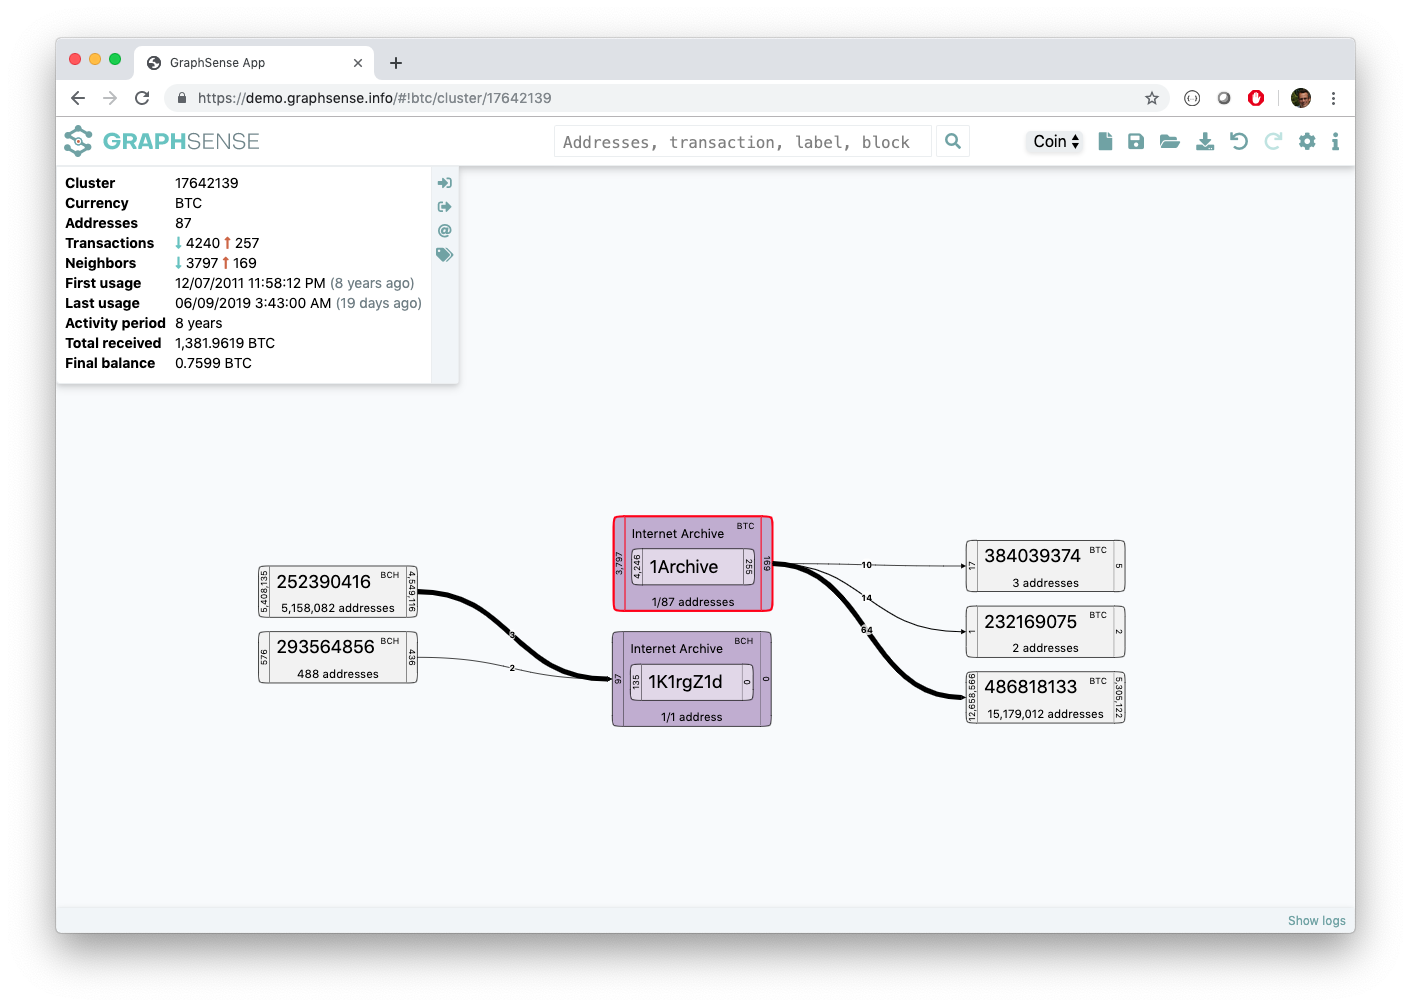
\includegraphics[width=1.7cm]{\imgpath/dashboard.png}};
	\node (cliimage) at (cli) {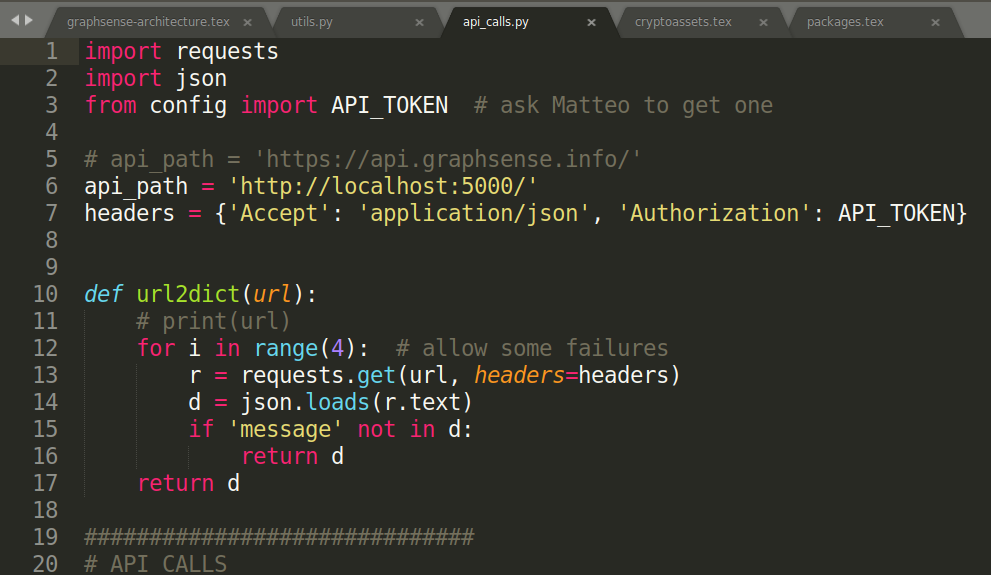
\includegraphics[width=1.8cm]{\imgpath/code.png}};


	% arrows
	\node[arr,  fill=white, minimum height = .7cm, minimum width = 1.2cm] at ($(raw.east)!0.34!(transformed.west)$){};
	\node[arr, fill = \ArrowColor, minimum height = 1.1cm] at ($(ingest.east)!0.43!(transform.west)$){};
	\node[arr, fill = \ArrowColor, minimum height = 1.1cm] at ($(sources.east)!0.43!(ingest.west)$){};
	\node[arr, fill = \ArrowColor, rotate = 90, minimum height = .6cm] at ($(raw.north)!0.8!(cli.south)$){};
	\node[arr, fill = \ArrowColor, rotate = 90, minimum height = .6cm] at ($(transformed.north)!0.8!(dashboard.south)$){};

	\node (spark) at (-0.05, 0.04) {
\includegraphics[width=.5cm]{\imgpath/spark.png}};


\end{tikzpicture}

\end{document}